\documentclass[eng,printmode]{mgr}

\usepackage{polski} %przydatne podczas składania dokumentów w j. polskim
\usepackage[utf8]{inputenc} %kodowanie znakĂłw, zaleĹĽne od systemu
\usepackage[T1]{fontenc} %poprawne składanie polskich czcionek

%pakiety do grafiki
\usepackage{graphicx}
\usepackage{subfigure}
\usepackage{psfrag}

\usepackage{amsmath}
\usepackage{amsfonts}

\usepackage{supertabular}
\usepackage{array}
\usepackage{tabularx}
\usepackage{hhline}
\usepackage{float}
\usepackage{showlabels}

\newcommand{\R}{I\!\!R} %symbol liczb rzeczywistych, działa tylko w trybie matematycznym
\newtheorem{theorem}{Twierdzenie}[section] %nowe otoczenie do składania twierdzeń

\title{Aplikacja do identyfikacji i rozpoznawania twarzy użytkownika w celu zabezpieczenia dostępu przy użyciu technologii Qt}
\engtitle{Qt based secure access application using face detection and identification}
\author{Dominik Guderski}
\supervisor{dr inż. Andrzej Rusiecki, W-4/K-9}
\graphicspath{ {../img/}}

\field{Automatyka i Robotyka (AIR)}
\specialisation{Technologie Informacyjne w Systemach Automatyki (ART)}
\begin{document}
\bibliographystyle{plabbrv}

\maketitle
\dedication{6cm}{Projekt dedykuję rodzicom.}

\tableofcontents


\chapter{Wstęp}
Rozpoznawanie twarzy jako technika biometryczna służąca do identyfikacji osób wykształciła się jako obiekt zainteresowań naukowców w latach osiemdziesiątych XX wieku. Pierwsze komercyjne systemy powstały w latach dziewięćdziesiątych XX wieku\cite{historyreco}.

Główną cechą rozpoznawania twarzy jest bezinwazyjność. Wystarczy spojrzenie w obiektyw. Systemy wykrywające i rozpoznające twarz wymagają szczególnych warunków otoczenia do poprawnego działania. Zmiany oświetlenia, położenia twarzy względem urządzenia rejestrującego mogą w znaczny sposób zaburzyć działanie algorytmu detekcji i rozpoznawania twarzy. W skrajnych przypadkach zmiana oświetlenia lub zmiana położenia twarzy względem urządzenia rejestrującego może uniemożliwić działanie algorytmów.
\section{Cel i zakres programu}

Niniejsza praca dotyczy praktycznego zagadnienia zabezpieczania dostępu do zasobów. Autor zaimplementował dwuelementowe uwierzytelnianie. Sprawdzana jest znajomość zdefiniowanego wcześniej hasła dla danego użytkownika oraz porównywana jest twarz odczytana z kamery z informacjami zawartymi w bazie danych. Moduł uwierzytelniania i obsługi informacji o użytkownikach został zaimplementowany przez autora od podstaw. Za bazę do stworzenia algorytmu identyfikacji oraz rozpoznawania twarzy posłużyła biblioteka OpenCV. Głównym celem było stworzenie programu, który realizowałbym zadanie kontrolowania dostępu do zasobów poprzez rozpoznawanie twarzy w czasie rzeczywistym porównując z twarzami wzorcowymi oraz sprawdzanie znajomości hasła.

\section{Układ pracy}

We wstępie został opisany temat pracy, poruszone w niej zagadnienia oraz problemy związane z tematyką. W rozdziale drugim przedstawiono opis zagadnień teoretycznych związanych z tematem pracy. Opisano metody oraz biblioteki użyte w procesie realizacji założeń projektu. W podsumowaniu znajdują się wnioski czego udało się dokonać, czego udało się uniknąć i co sprawiło problemy. Podana też została propozycja jednej ze ścieżek dalszego rozwoju aplikacji.
\section{Koncepcja rozwiązania problemu}

By zrealizować idee uwierzytelniania użytkownika na podstawie hasła oraz zdjęcia twarzy potrzebne są dwa elementy. Baza danych zawierająca nazwę użytkownika i hasło, oraz baza danych zawierająca wzorcowe zdjęcia twarzy powiązane z użytkownikiem. Oczywiście kwestią implementacyjną jest czy owe bazy będą jednym obiektem, czy też dwoma. W wypadku opisywanego projektu wybrane zostało podejście dwóch baz. Oczywiście obie te bazy są ze sobą synchronizowane i razem tworzą koncepcyjnie jedną bazę danych, nazywaną dalej bazą danych użytkowników.
\subsection{Przechowanie nazwy użytkownika i hasła}

Uwierzytelnianie użytkowników wymaga bazy danych. Owa baza została zrealizowana przy pomocy dwóch elementów. Pierwszy z nich to plik .face\_recognizerrc, który przechowuje nazwę użytkownika oraz zakodowane hasło, w zdefiniowanym przez program formacie(zdefiniowanym w taki sposób by ułatwić przetwarzanie pliku przez program). Format ten ma postać:\\
::nazwa\_użytkownika::zakodowane\_hasło::\\
::nazwa\_użytkownika2::zakodowane\_hasło2:: \\
\begin{figure}[placement h]
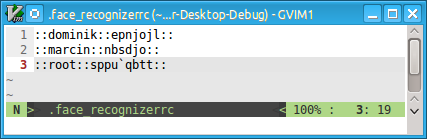
\includegraphics{face}
\caption{Format pliku przechowującego login i hasło}
\end{figure}

Czyli dla każdego użytkownika przeznaczona jest jedna linia w pliku. Nazwa użytkownika jest umieszczona w sposób niezakodowany, natomiast hasło umieszczone jest w sposób zakodowany prostym wariantem szyfru Cezara. Celem autora nie była implementacja nietrywialnego algorytmu szyfrowania hasła, ponieważ przyjęte zostało założenie, iż pliki konfiguracyjne programu są umieszczone w bezpiecznej lokalizacji. Można to osiągnąć uruchamiając program z konta administratora(wtedy pliki konfiguracyjne mogą zostać umieszczone w katalogu chronionym przed odczytem przez innych użytkowników niż administrator).
\\

Innym rozwiązaniem jest uruchomienie programu w dowolnym miejscu, jednak ograniczenie interface'u poprzez który użytkownicy programu mogą sterować programem. Takim ograniczeniem może być odpowiednie przygotowanie systemu operacyjnego, tak by uruchomiony program zajmował całą dostępna przestrzeń ekranu. Dodatkowo użytkownik ma do dyspozycji ekran dotykowy by móc sterować działaniem programu. Nie ma możliwości przełączenia czy też włączenia innego procesu w systemie. Takie podejście może zostać zastosowane przy projektowaniu interface'u do sterowania inteligentnym budynkiem lub pomieszczeniem.
\subsection{Przechowywanie wzorcowych zdjęć twarzy}

Program oprócz wspomnianego pliku przechowującego dane tekstowe tworzy także katalog .face\_recognizer. W tym katalogu dla każdego użytkownika z wyjątkiem użytkownika root(administrator) istnieje katalog o nazwie odpowiadającej nazwie użytkownika.
.face\_recognizer/\\
\textbullet nazwa\_użytkownika/\\
\textbullet nazwa\_użytkownika2/\\
Katalog ten w momencie dodania użytkownika do bazy danych jest wypełniany dostarczonymi przez użytkownika  pięcioma wzorcowymi zdjęciami twarzy. Wzorce te w momencie próby uzyskania dostępu do systemu przez użytkownika są porównywane z obrazem wykrytej twarzy z kamery podłączonej do systemu.\\
\begin{figure}[placement h]
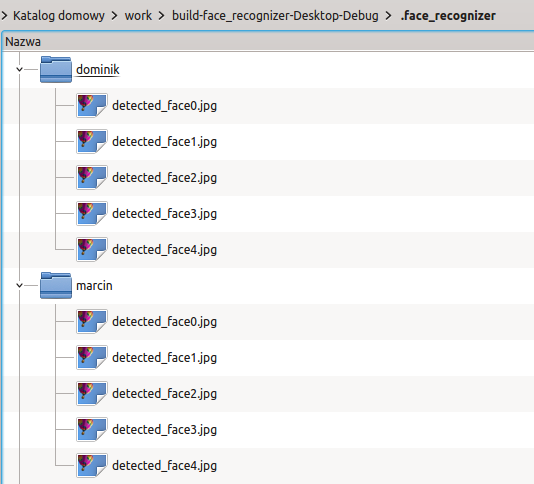
\includegraphics[scale=0.5]{dir}
\caption{Format katalogu przechowującego wzorcowe zdjęcia twarzy }
\end{figure}
\subsection{Konto administratora}

Wyjątkowym przypadkiem, o którym należy wspomnieć jest konto administratora(login: root, domyślne hasło: pass). Owe konto jako jedyne jest dostępne już przy pierwszym uruchomieniu programu z domyślnym hasłem dostarczonym razem z programem. Bardzo ważna ze względów bezpieczeństwa jest zmiana domyślnego hasła. Wymaganiem stawianym administratorowi podczas procedury uwierzytelniania jest podanie prawidłowego hasła. Nie jest sprawdzany obraz z kamery. Oprócz tego konto root nie posiada katalogu root w katalogu .face\_recognizer/, gdyż nie jest on potrzebny. Konto administratora jest potrzebne by dodawać i usuwać użytkowników.

\subsection{Detekcja i rozpoznawanie twarzy}

W celu detekcji i rozpoznawania twarzy została użyta biblioteka OpenCV. Detekcja twarzy odbywa się przy użyciu funkcji Haar-like, umożliwiającej dość dobrą i szybką detekcję obiektów. Rozpoznawanie jest zrealizowane za pomocą metody EigenFace.

Podstawowy problem- szybkość przetwarzania obrazu, który zależy od mocy obliczeniowej
komputera oraz zaimplementowanego algorytmu. Ważna kwestią jest poprawność wykrywania
twarzy. W wypadku gdy algorytm wykryje twarz w miejscu gdzię rzeczywiście jej nie ma może
to prowadzić do błędnego działania programu, a także oznacza marnowanie zasobów. Z tego powodu w programie został przyjęty minimalny rozmiar wykrytej twarzy (50x50 pikseli). Wykryte obiekty mniejsze od tej granicznej wielkości nie są przetwarzane.

Takie podejście nie rozwiązuje jednak wszystkich problemów. Nadal może dojść do sytuacji, w której algorytm wykryje obszar obrazu twierdząc, że jest to twarz podczas gdy nie będzie to twarz.\\
\begin{figure}[placement h]
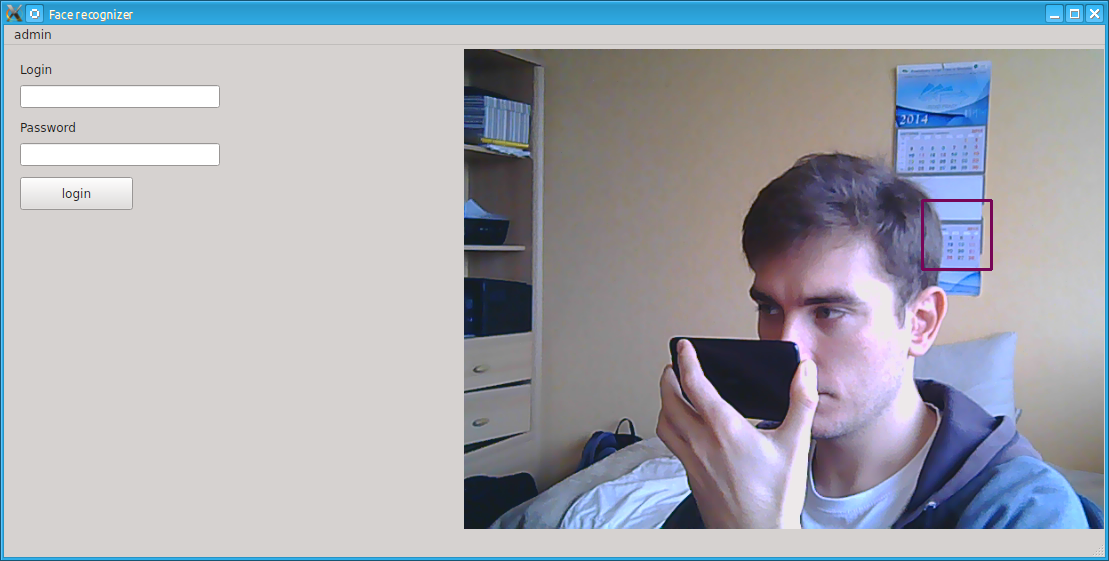
\includegraphics[scale=0.4]{facenotdetected}
\caption{Twarz wykryta w niewłaściwym miejscu}
\end{figure}

Program, który wykorzystuje funkcję Haar-like bazujący na rozpoznawaniu założonych wzorców jest szybki i dobrze pracuje w czasie rzeczywistym, jednak losowe zakłócenia w obrazie wejściowym(np. zła jakość obrazu, oświetlenie, niejednolite tło) mogą prowadzić do wskazania fragmentu obrazu nie zawierającego twarzy.\\

Podobny błąd może powodować umieszczenie przed obiektywem kamery ekranu LCD, na którym wyświetlane jest zdjęcie twarzy. Owym ekranem może być telefon komórkowy, tablet. Co oznacza, że podobny efekt działania algorytmu może być osiągnięty poprzez umieszczenie np. manekina przed obiektywem kamery.\\
\begin{figure}[placement h]
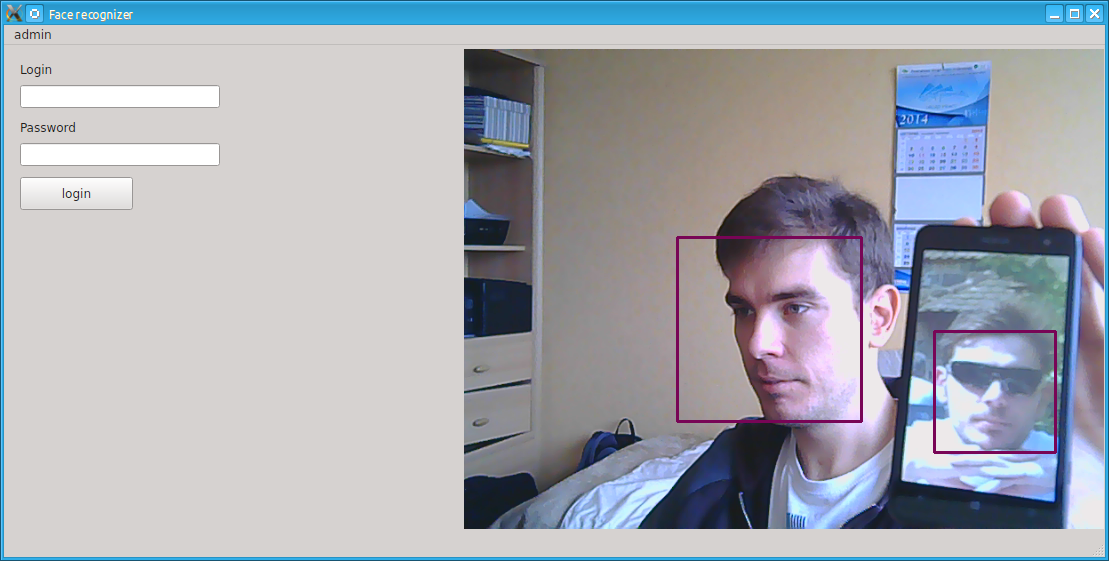
\includegraphics[scale=0.4]{cellphone}
\caption{Twarz wykryta na ekranie LCD}
\end{figure}

Dużym wyzwaniem dla algorytmu wykrywającego jak i rozpoznającego twarz są także obroty twarzy względem kamery. Kolejnymi elementami są wszelkie ozdoby, czy też części garderoby. Okulary, czapka, zarost, tatuaże, kolczyki mogą w znaczący sposób zaburzyć owal głowy. Dla algorytmów wykrywających na podstawie koloru skóry obrót nie jest dużym problemem, jednak dla algorytmów opierających się na cechach twarzy różny jej kąt względem kamery stanowi wyzwanie.\\
\begin{figure}[placement h]
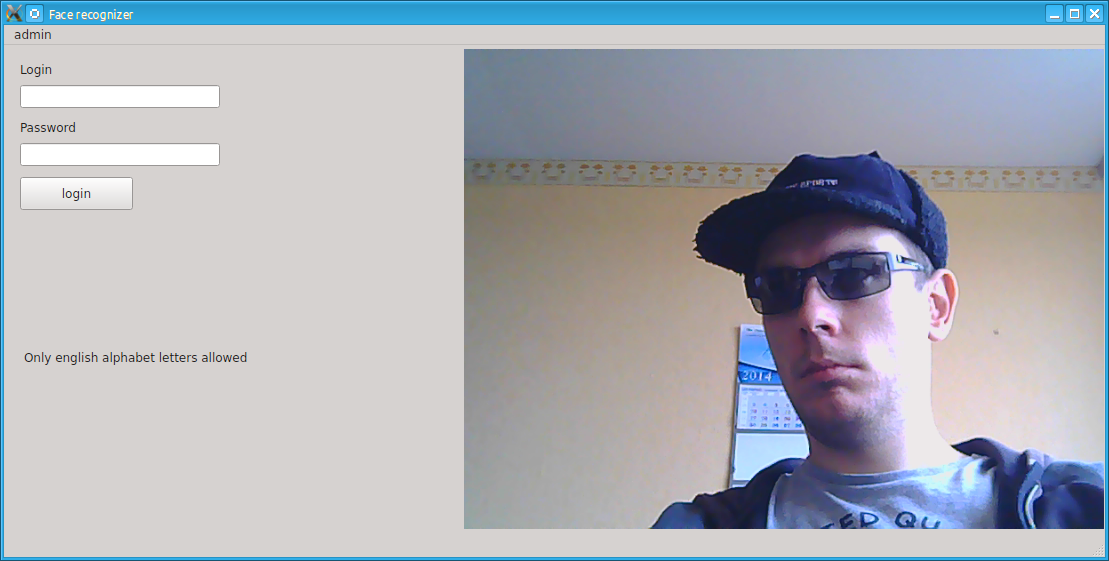
\includegraphics[scale=0.4]{hatnotdet}
\caption{Twarz nie wykryta- czapka i okulary}
\end{figure}

Detekcja jak i rozpoznawanie twarzy nie pozostają obojętne na warunki świetlne, w których wykonywane jest pobieranie obrazu przez kamerę. Oprócz samego natężenia, równomierności oświetlenia jest jeszcze kwestia jakości urządzenia pobierającego obraz. Istnieją kamery, które posiadają moduły wyrównywanie natężenia oświetlenia na pobranym obrazie realizowane zarówno sprzętowo jak i poprzez wbudowane oprogramowanie. Nie bez znaczenia pozostaje rozdzielczość kamery. Niska sprawia, że obraz jest zniekształcony co utrudnia w sposób znaczny działanie algorytmów detekcji czy rozpoznawania. Kolejnymi problemami technicznymi związanymi z budżetowymi urządzeniami pobierającymi obraz są problemy z auto fokusem. Jednym z rozwiązań jest stosowanie wysokiej jakości kamery. Choć i tutaj w skrajnych przypadkach(bardzo małe natężenie światła) otrzymany obraz nie będzie nadawał się do opisywanych algorytmów. Skrajnym rozwiązaniem jest stosowanie kamery termowizyjnej. W wypadku takich urządzeń użytkownik zostaje uniezależniony od natężenia światła, dzięki czemu problemy opisywane wyżej nie występują. Wadą tego rozwiązania jest koszt kamery termowizyjnej. W chwili przygotowywania projektu koszt kamery termowizyjnej został oszacowany na 2 rzędy wielkości wyższy aniżeli koszt standardowej kamery. Przyjmuje się, że do działania opisywanego systemu dane wejściowe dostarczane przez urządzenie pobierające obraz są dobrej jakości.
\chapter{Podstawy teoretyczne}


\section{Model barw}

RGB – jeden z modeli przestrzeni barw, opisywanej współrzędnymi RGB. Jego nazwa powstała ze złożenia pierwszych liter angielskich nazw barw: R – red (czerwonej), G – green (zielonej) i B – blue (niebieskiej), z których model ten się składa. Jest to model wynikający z właściwości odbiorczych ludzkiego oka, w którym wrażenie widzenia dowolnej barwy można wywołać przez zmieszanie w ustalonych proporcjach trzech wiązek światła o barwie czerwonej, zielonej i niebieskiej.

Z połączenia barw RGB w dowolnych kombinacjach ilościowych można otrzymać szeroki zakres barw pochodnych, np. z połączenia barwy zielonej i czerwonej powstaje barwa żółta. Do przestrzeni RGB ma zastosowanie synteza addytywna, w której wartości najniższe oznaczają barwę czarną, najwyższe zaś – białą. Model RGB jest jednak modelem teoretycznym, a jego odwzorowanie zależy od urządzenia (ang. device dependent), co oznacza, że w każdym urządzeniu każda ze składowych RGB może posiadać nieco inną charakterystykę widmową, a co za tym idzie, każde z urządzeń może posiadać własny zakres barw możliwych do uzyskania.

Model RGB miał pierwotnie zastosowanie do techniki analogowej, obecnie ma również do cyfrowej. Jest szeroko wykorzystywany w urządzeniach analizujących obraz (np. aparaty cyfrowe, skanery) oraz w urządzeniach wyświetlających obraz (np. telewizory, monitory komputerowe).

Zapis koloru jako RGB często stosuje się w informatyce (np. palety barw w plikach graficznych, w plikach HTML). Najczęściej stosowany jest 24-bitowy zapis kolorów (po 8 bitów na każdą z barw składowych), w którym każda z barw jest zapisana przy pomocy składowych, które przyjmują wartość z zakresu 0-255. W modelu RGB wartość 0 wszystkich składowych daje kolor czarny, natomiast 255 – kolor biały. W rzadszych przypadkach stosuje się model, w którym przypada po 12 lub 16 bitów na każdą ze składowych, co daje dużo większe możliwości przy manipulowaniu kolorem\cite{wikirgb}. \\
Kolor RGB można obliczyć ze wzoru:
\\
\text{numer koloru} = R * 65536 + G * 256 + B\\
gdzie R, G i B przyjmują wartość od 0 do 255.\\

\begin{figure}[placement h]
\includegraphics[scale=1]{rgb}
\caption{Przestrzeń RGB}
\end{figure}

Oprócz wspomnianego modelu istnieje także BGR(używany np. w OpenCV), który różni się od wyżej opisanego kolejnością następowania po sobie 3 bazowych kolorów.
\section{Identyfikacja twarzy}

Klasyfikator Haar'a jest to element zaimplementowany w bibliotece OpenCV. Może służyć do wykrywania obiektów na obrazie. W projekcie posłużył do wykrywania twarzy. Klasyfikator bazuje na kaskadzie stworzonej z wektora uczącego. Kaskada ta, w formie pliku XML z danymi jest dostarczana jako część biblioteki OpenCV. Bazując na zaimplementowanym w bibliotece algorytmie oraz dostarczonym plik z ciągami uczącymi pozwala na wykrycie twarzy na zdjęciu. Wyszukiwanie dla całego obrazu wejściowego realizowana jest przy pomocy koncepcji okna. Prostokąt o szerokości i wysokości mniejszej niż obraz wejściowy przesuwany jest po obrazie wejściowym. Algorytm wyszukiwania obiektu jest realizowany na tak zdefiniowanym przez prostokąt fragmencie obrazu. Klasyfikator można zakwalifikować jako algorytm o dużym obciążeniu, ale także o dużej dokładności działania.

\section{Szyfrowanie hasła}

Szyfr Cezara (zwany też szyfrem przesuwającym, kodem Cezara lub przesunięciem Cezariańskim) – w kryptografii jedna z najprostszych technik szyfrowania. Jest to rodzaj szyfru podstawieniowego, w którym każda litera tekstu jawnego (niezaszyfrowanego) zastępowana jest inną, oddaloną od niej o stałą liczbę pozycji w alfabecie, literą (szyfr monoalfabetyczny), przy czym kierunek zamiany musi być zachowany. Nie rozróżnia się przy tym liter dużych i małych. Nazwa szyfru pochodzi od Juliusza Cezara\cite{szyfrcezara}.\\
\begin{figure}[placement h]
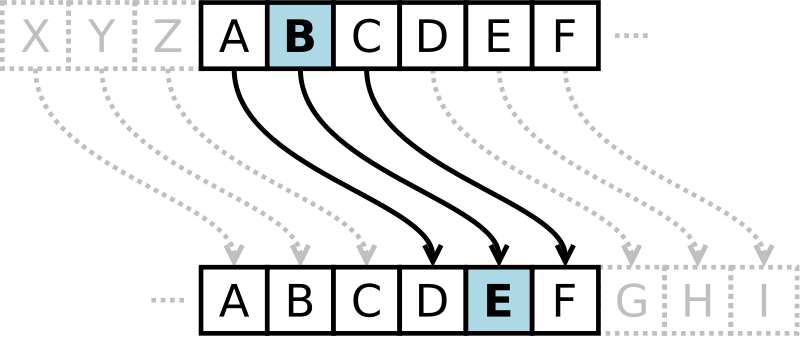
\includegraphics[scale=0.4]{caesar}
\caption{Szyfr Cezara}
\end{figure}

Użyta w projekcie metoda szyfrowania rozróżnia duże i małe litery i przypisuje im wagi zgodne z tablicą ASCII. Przesunięcie wynosi 1. Szyfrowanie zostało zastosowane w projekcie do celów innych niż najczęściej rozumiane zabezpieczenie informacji. Przyjęte jest założenie, że użytkownicy, którzy próbują uzyskać dostęp do zasobów poprzez opisywany system nie mogą uzyskać dostępu do pliku, w którym przechowywane są dane dotyczące nazw użytkowników i ich haseł. Takie ograniczenie może wynikać z ograniczeń w interfejsie dostępnym dla użytkownika systemu, lub wprost z konstrukcji systemu operacyjnego, w którym uruchamiana jest aplikacja(można założyć, że aplikacja uruchomiona jest w systemie linux z uprawnieniami użytkownika root i w katalogu domowym tego użytkownika, z czego wynika, że żaden użytkownik poza użytkownikiem root domyślnie nie będzie miał dostępu do czytania z bazy danych programu). Wprowadzenie szyfrowania zostało podyktowane możliwością przypadkowego otwarcia pliku przez administratora systemu. W takim wypadku administrator nie odczyta prawdziwego hasła. Dopiero celowa chęć odszyfrowania hasła może sprawić, że odczyta hasło innego użytkownika.

Algorytm szyfrowania zastosowany w kodzie Cezara bywa fragmentem bardziej złożonych systemów szyfrowania, takich jak szyfr Vigenère'a. Współcześnie szyfru Cezara używa się z przesunięciem 13 (ROT13), będącego prostym i szybkim sposobem na ukrycie treści.
\chapter{Opis programu}
\section{Użyte technologie}

Program został stworzony w systemie operacyjnym Linux 3.13.0-39-generic \#66-Ubuntu SMP, Ubuntu 14.04 w języku C++(ISO/IEC C++ 2003) przy użyciu kompilatora g++ (Ubuntu 4.8.2-19ubuntu1) 4.8.2. Środowiskiem służącym do projektowania graficznego interfejsu użytkownika był program Qt Creator 3.0.1 oparty na bibliotece Qt 5.2.1. Oprócz wspominanych elementów zastosowane zostały biblioteki OpenCV 2.4.8, boost 1.54.0.1 przy tworzeniu kodu produkcyjnego- przeznaczonego do wytworzenie oprogramowania. Oprócz tego pomocniczo przy tworzeniu testów jednostkowych został użyty pakiet gmock 1.7.0.
\subsection{OpenCV}

OpenCV to otwarta biblioteka stworzona przez Intel. W momencie tworzenia projektu udostępnione był interfejs biblioteki w językach C++, C, Python, Java. Biblioteka może być używana w systemie Windows, Linux, Mac OS, iOS oraz Android. Pracę nad biblioteką zostały rozpoczęte w 1999 roku. Wersja dojrzała została udostępniona w 2006 roku. Biblioteka jest wydawana na licencji BSD(Berkeley Software Distribution License). Ta bardzo liberalna licencja pozwala nie tylko na modyfikacje kodu biblioteka, ale także rozprowadzanie go w takiej postaci. Pozwala także na rozprowadzanie produktu bez postaci źródłowej czy wręcz włączenie do zamkniętego oprogramowania, pod warunkiem załączenia do produktu informacji o autorach oryginalnego kodu i treści licencji.
\subsection{Boost}

Kolekcja bibliotek programistycznych poszerzających możliwości języka C++, objętych liberalną licencją(Boost Software License), która umożliwia użycie ich w dowolnym projekcie.

Dzięki restrykcyjnemu systemowi recenzowania i kontroli jakości, biblioteki Boost są poważane ze względu na ich wysoką jakość oraz często stawiane za wzorcowy przykład nowoczesnego projektowania i programowania w C++. Dziedziny zastosowania Boost są bardzo szerokie, pakiet dostarcza m.in. biblioteki ogólnego przeznaczenia (inteligentne wskaźniki, wyrażenia regularne), biblioteki stanowiące warstwę abstrakcji dla systemu operacyjnego (obsługa systemów plików czy wielowątkowości), jak i narzędzia przeznaczone głównie dla innych twórców bibliotek i zaawansowanych programistów języka C++ (np. biblioteka metaprogramowania MPL). Kilka bibliotek wchodzących w poczet Boost zostało włączonych do pierwszego raportu technicznego komitetu standaryzacyjnego C++ (w jego skład wchodzi wielu spośród twórców Boost)\cite{wikiboost}.
\subsection{Qt}

Zestaw przenośnych bibliotek i narzędzi programistycznych dedykowanych dla języków C++, QML i Java. Ich podstawowym składnikiem są klasy służące do budowy graficznego interfejsu programów komputerowych, począwszy od wersji 4.0 Qt zawiera też narzędzia do tworzenia programów konsolowych i serwerów.

Środowisko Qt jest dostępne dla platform: X11 (m.in. GNU/Linux, BSD, Solaris), Windows, Mac OS X, Haiku oraz dla urządzeń wbudowanych opartych na Linuksie (Qt Extended), Windows CE, Symbian, Android. Qt jest podstawą dla m.in. uniksowego środowiska graficznego KDE oraz uniksowych wersji komunikatora internetowego Skype i programu Google Earth.

Biblioteki Qt dostępne są w języku C++ i Java; mogą też być wykorzystywane w programach napisanych w innych językach, m.in. Ada (QtAda), C\# (Qyoto/Kimono), Pascal, Perl (Perl Qt4), PHP (PHP-Qt), Ruby (QtRuby) i Python (PyQt). Charakteryzują się w pełni obiektową architekturą.
Licencje LGPL (v. 2.1), GPL (v. 3.0), komercyjna\cite{wikiqt}.
\subsection{Gmock}

Biblioteka do testów jednostkowych oprogramowania dla języka C++, bazująca na architekturze xUnit. Jest wydawana na licencji BSD 3. Może być używana na wielu platformach: Linux, Windows, Mac OS X.

\section{Konfiguracja środowiska programistycznego Qt}

Przed przystąpieniem do pisania projektu korzystającego z biblioteki OpenCV w technologii qt powinno się przeprowadzić kilka operacji, by kompilacja jak i linkowanie przebiegało pomyślnie. Zakładając, że w systemie są zainstalowane wyżej wspomniane biblioteki oraz oprogramowanie Qt Creator:

Po uruchomieniu programu Qt Creator należy z menu kontekstowego File wybrać opcję New file or project, a następnie Applications/Qt Widgets Application\\
\begin{figure}[placement h]
\includegraphics[scale=0.5]{newproject}
\caption{Nowy projekt Qt}
\end{figure}
\\
Po wybraniu nazwy oraz lokalizacji projektu, należy przejść do katalogu z projektem i otworzyć plik nazwa\_projektu.pro:\\
\begin{figure}[placement h]
\includegraphics[scale=0.5]{blankprofile}
\caption{Czysty plik konfiguracyjny pro}
\end{figure}\\
i dodać linię:\\
\textbf{LIBS += `pkg-config opencv --libs`}\\
Podobną komendę stosuje się w pliku konfiguracyjnym dla innych bibliotek. Tak wygląda plik pro zrealizowanego programu.\\
\begin{figure}[placement h]
\includegraphics[scale=0.5]{fullproconfig}
\caption{Plik pro zrealizowanego projektu}
\end{figure}\\


\section{Podręcznik użytkownika}
Program został napisany przez Dominik Guderskiego, jako element projektu inżynierskiego. Opracowanie zostało napisane 30.11.2014 r.

Program do działania w folderze, w którym jest uruchamiany potrzebuje pliku haarcascade\_frontalface\_alt.xml oraz kamery poprawnie podłączonej i rozpoznanej przez system operacyjny. Po spełnieniu powyższych warunków i uruchomieniu programu ukazuje się okno:\\

\begin{figure}[placement h]
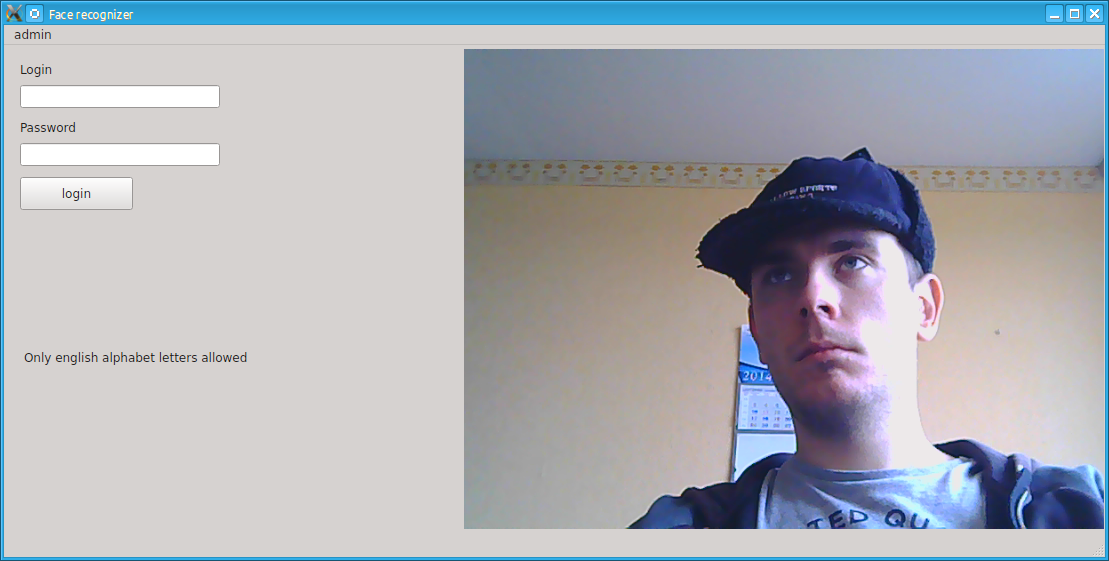
\includegraphics[scale=0.4]{programstarted}
\caption{Główne okno programu}
\end{figure}

Każde pole przyjmujące informacje tekstowe od użytkownika(pola tekstowe takie jak login, password) przyjmują wyłącznie znaki należące do angielskiego alfabetu. Można wprowadzić inne znaki do samego pola formularza, jednak taki napis nie będzie dalej przetwarzany. By zalogować się do systemu należy wpisać poprawną nazwę użytkownika(login) oraz hasło.  Oprócz konta root(administratora) wymagane jest także by na obrazie z kamery widocznym w prawej części okna logowania została wykryta twarz i by ta twarz została rozpoznana jako ta sama, która znajduje się w bazie danych przypisana do użytkownika, który próbuje się zalogować.

W lewym górnym rogu okna dostępne jest menu admin, w którym zawarte są funkcje administracyjne:\\
\begin{figure}[placement h]
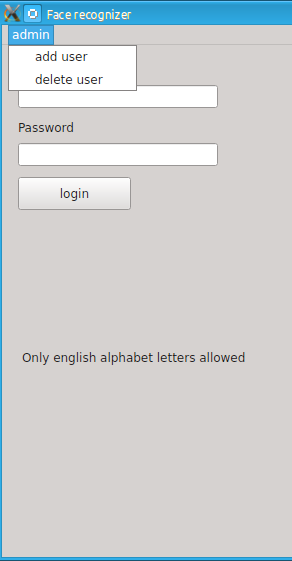
\includegraphics[scale=0.4]{contextmenu}
\caption{Menu kontekstowe}
\end{figure}\\

Po wybraniu opcji add user(dodaj użytkownika) otwiera się nowe okno umożliwiające dodanie nowego użytkownika:\\
\begin{figure}[placement h]
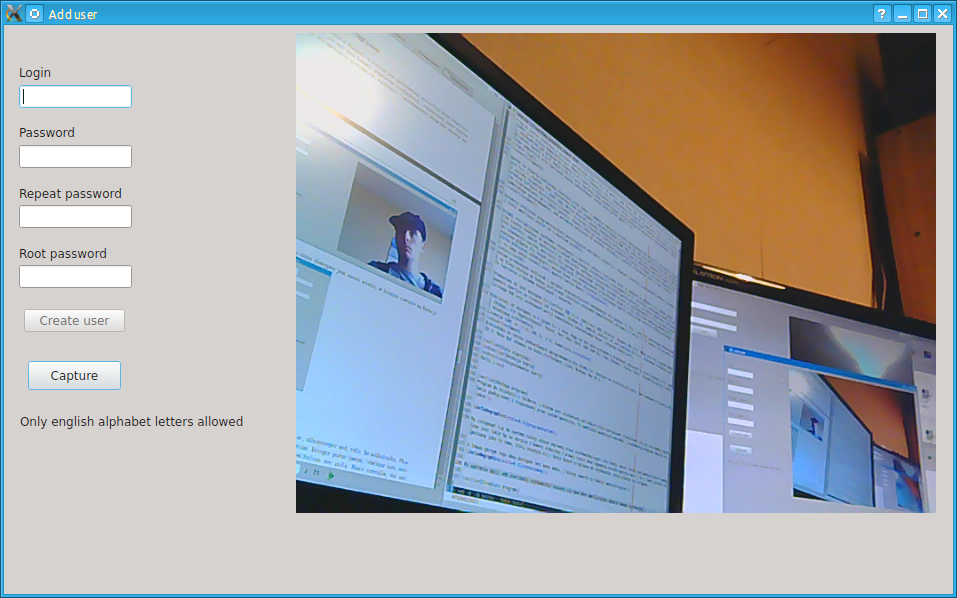
\includegraphics[scale=0.4]{adduser}
\caption{Okno dodania użytkownika}
\end{figure}\\
Aby dodać użytkownika należy wykonać 5 zdjęć, które będą używane przy logowaniu do systemu(sprawdzanie czy twarz widniejąca na obrazie kamery w momencie logowania jest tą samą która została dodana do bazy danych dla danego użytkownika). Kiedy na obrazie po prawej stronie okna będzie widoczny prostokąt otaczający twarz użytkownika należy wcisnąć przycisk Capture. Czynność należy powtórzyć 5 razy. Gdy to zadanie zostanie wykonane pomyślnie przycisk Create user stanie się aktywny i będzie możliwe stworzenie nowego użytkownika po uzupełnieniu wszystkich pól formularza. Należy wpisać nazwę nowego użytkownika, hasło, powtórzyć hasło oraz hasło administratora(konto root). Po wykonaniu tych czynności i wciśnięciu przycisku Create user, jeśli nie pojawiły się inne błędy(błąd zapisu do pliku, ciąg znaków w polu password i repeated password nie są równe) nowy użytkownik zostanie dodany do bazy danych.

Analogicznie skonstruowane zostało okno, które otwiera się gdy w głównym oknie programu z menu kontekstowego zostanie wybrana opcja delete user. Tutaj dane tekstowe, które podawane są przez użytkownika to: login(nazwa użytkownika) i root password(hasło administratora). W tym oknie nie ma obrazu z kamery, ponieważ do uwierzytelniania konta administratora nie używa się obrazu z kamery. Jeśli wszystkie dane zostały wpisane poprawnie i użytkownik istnieje w bazie usunięcie powiedzie się.\\
\begin{figure}[placement h]
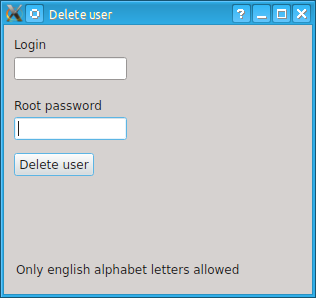
\includegraphics[scale=0.7]{deluser}
\caption{Okno usunięcia użytkownika}
\end{figure}

\begin{figure}[placement H]
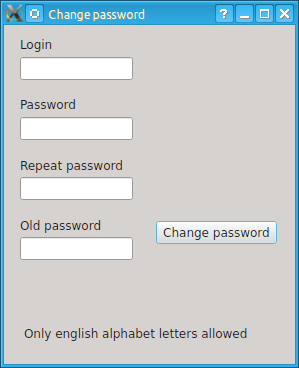
\includegraphics[scale=0.6]{authenticated}
\caption{Zmiana hasła}
\end{figure}
Gdy w głównym oknie programu wpiszemy poprawne dane uwierzytelniające uzyskamy dostęp do chronionych zasobów. Taka akcja może spowodować uruchomienie dowolnego okna, otwarcie dowolnego dokumentu. Do celów demonstracyjnych zostało wprowadzone okno pozwalające zmienić hasło użytkownika:\\

Po poprawnym wypełnieniu wszystkich pól następuje zmiana dotychczasowego hasła na nowe dla wybranego użytkownika.
\section{Struktura programu}
Program można podzielić koncepcyjnie na dwa elementy. Warstwę prezentacji i warstwę logiczną. Warstwę prezentacji stanowi kod odpowiedzialny za tworzenie i obsługę graficznego interfejsu użytkownika. Natomiast warstwa logiczna to klasy realizująca potrzebne algorytmy: komunikacje z bazą danych, kodowanie hasła czy też rozpoznawanie twarzy. Takie podejście jest zgodne z paradygmatem pisania oprogramowania dla systemów z rodziny Linux.\\
\begin{figure}[placement h]
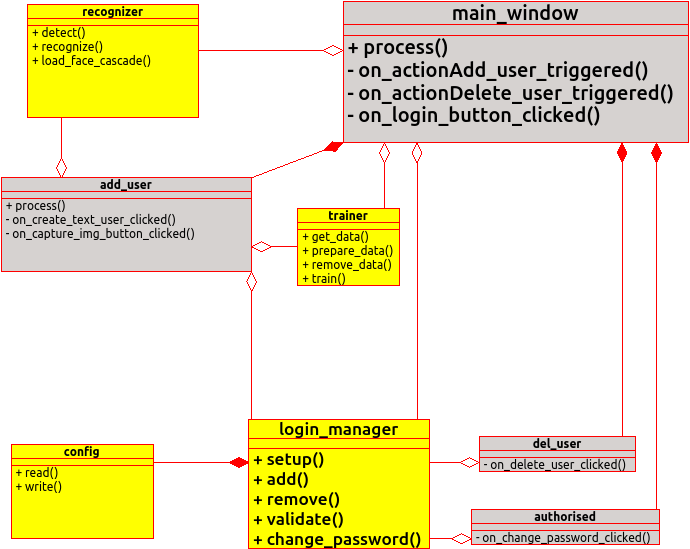
\includegraphics[scale=0.7]{classdiag}
\caption{Diagram klas programu}
\end{figure}\\
Jeżeli zajdzie potrzeba, można stworzyć graficzny interfejs użytkownika w zupełnie odmiennej technologii niż użyta w tym projekcie. Dzięki oddzieleniu dwóch warstw prezentacji i logicznej taka potrzeba może być zrealizowana w relatywnie krótkim czasie. Będzie wymagać mało prac reorganizujących kod.

Kolejną zaletą takiego rodzaju modularności kodu jest łatwość testowania. Począwszy od zautomatyzowanych testów jednostkowych, które w swoich scenariuszach testowych mogą tworzyć instancje poszczególnych klas wywoływać na nich metody ich interfejsów po czym sprawdzać wyniki. Istnieją nawet propozycje i możliwości zautomatyzowanego testowania wszystkich metod danej klasy, a nie tylko jej interfejsu jednak nie są one tak rozpowszechnione. Także testy manualne aplikacji, gdy uruchamiana z linii komend i odpowiednio dostosowana do scenariusza testowego mogą przebiegać sprawniej niż z graficznym interfejsem użytkownika.

\chapter{Testowanie projektu}

Testowanie było dwuetapowe. Na etapie tworzenie implementacji warstwy logicznej równolegle z tworzenie implementacji powstawały testy jednostkowe pozwalające wykryć ewentualne błędy. Oprócz tego po napisaniu warstwy logicznej dodany został kod odpowiadający za warstwę prezentacji. W dużej mierze ten kod był testowany manualnie przez użytkownika. Wyniki testów całości można podzielić na trzy grupy:
\begin{itemize}
\item{Testowanie funkcjonalności uwierzytelniania kodem tekstowym i zarządzania użytkownikami}
\item{Testowanie algorytmu wykrywającego twarz}
\item{Testowanie algorytmu rozpoznającego twarz}
\end{itemize}

\section{Testowanie funkcjonalności uwierzytelniania kodem tekstowym i zarządzania użytkownikami}
Program poprawnie komunikuje się z bazą danych: dodaje, usuwa, modyfikuje użytkowników. Ponadto umożliwia zalogowanie się. Jedna z tych operacji może się nie powieść w wypadku, gdy np. system operacyjny nie pozwoli otworzyć jednego z plików, który należy do bazy danych.

\section{Testowanie algorytmu wykrywającego twarz}
Algorytm działa z dużą skutecznością. Nawet w trudnych warunkach oświetlenia(nierównomiernie doświetlone zdjęcie, małe natężenie oświetlenia) wykrywa z powodzeniem twarz. W testach manualnych autora, podczas obracania twarzy pod różnym kątem i stosowania różnego rodzaju oświetlenia oraz elementów ubioru(okulary, czapka) wykrywalność twarzy była na poziomie 80\%.\\
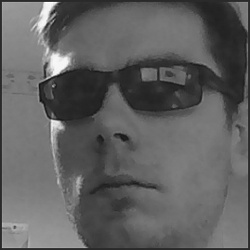
\includegraphics[scale=0.4]{cza1}
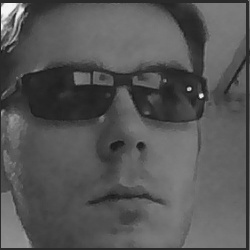
\includegraphics[scale=0.4]{cza2}
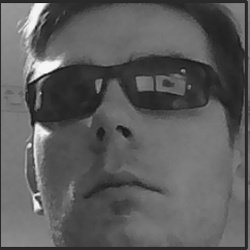
\includegraphics[scale=0.4]{cza3}\\
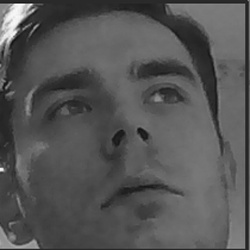
\includegraphics[scale=0.4]{detectedface0}
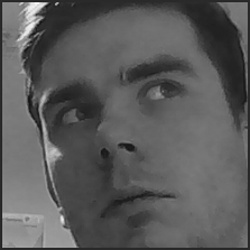
\includegraphics[scale=0.4]{detectedface1}
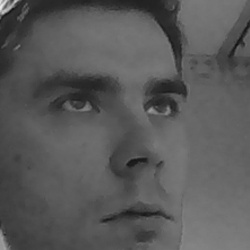
\includegraphics[scale=0.4]{detectedface2}\\

Choć pojawiają się sytuację, gdy przy trudnych warunkach twarz nie zostanie wykryta- brak prostokąta otaczającego twarz.\\
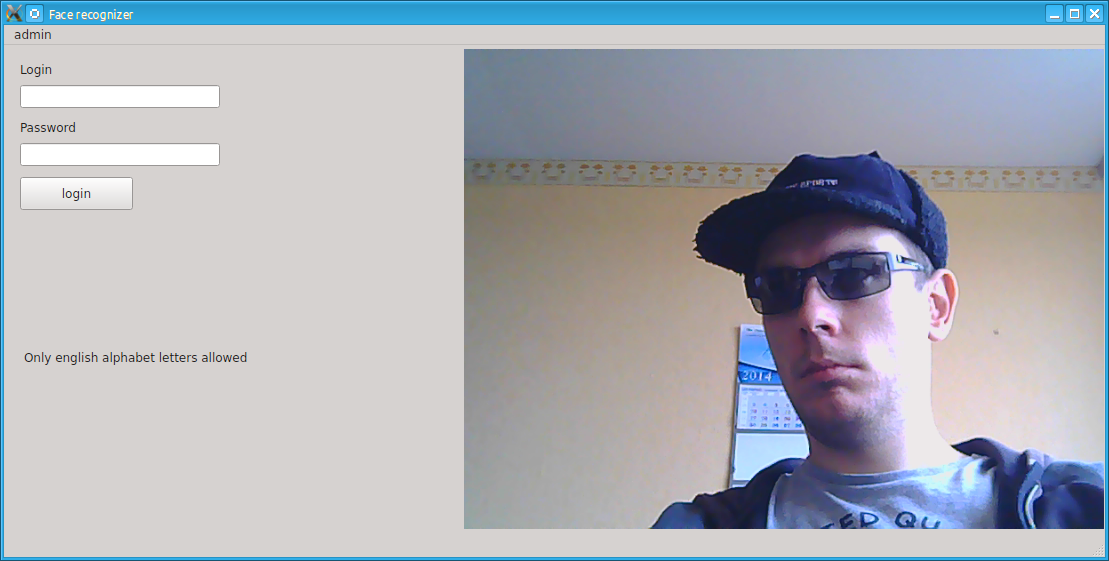
\includegraphics[scale=0.4]{hatnotdet}\\

W praktyce nie da się precyzyjnie wyznaczyć granicznego kąta obrotu twarzy względem obiektywu kamery gdy twarz przestaje być wykrywana. Bowiem oprócz wspomnianego parametru pojawia się wiele innych zmiennych- oświetlenie, cechy charakterystyczne danej twarzy, mimika czy ubiór.

\section{Testowanie algorytmu rozpoznającego twarz}
\chapter{Podsumowanie}
Efektem projektu jest aplikacja działająca w systemie graficznym zbudowana w oparciu o technologię Qt realizująca założenia i koncepcję projektu. System kontroli dostępu za pomocą hasła oraz biometrycznego zabezpieczenia- rozpoznawania twarzy został zrealizowany. Program identyfikuje twarze w czasie rzeczywistym. Program rozpoznaje twarze w czasie rzeczywistym. Przy kwestii rozpoznawania twarzy wpływ na skuteczność działania algorytmu mają warunku oświetlenia kąt nachylenia twarzy względem obiektywu kamery oraz odzież, ozdoby znajdujące się na twarzy użytkownika w czasie działania algorytmu.

\addcontentsline{toc}{chapter}{Bibliografia} %utworzenie w spisie treści pozycji Bibliografia
%\bibliography{bibliografia} % wstawia bibliografię korzystając z pliku bibliografia.bib - dotyczy BibTeXa, jeżeli nie korzystamy z BibTeXa należy użyć otoczenia thebibliography
\begin{thebibliography}{18}

\bibitem{masteringopencv} Daniel Lelis Baggio, Mastering OpenCV with Practical Computer Vision Projects
\bibitem{learningopencv} Adrian Kaehler, Gary Bradski, Learning OpenCV 2nd Edition
\bibitem{rafajlowicz09}  Ewaryst Rafajłowicz, Wojciech Rafajłowicz, Andrzej Rusiecki, Algorytmy przetwarzania obrazów i wstęp do pracy z biblioteką OpenCV
\bibitem{guiqt} Jasmin Blanchette, Mark Summerfield, C++ GUI Programming with Qt 4, Second Edition
\bibitem{cleancode} Robert C. Martin, Czysty kod. Podręcznik dobrego programisty
\bibitem{boost} http://www.boost.org/doc/
\bibitem{stl} http://www.cplusplus.com/reference/
\bibitem{opencv} http://docs.opencv.org/
\bibitem{facedetection} http://www.multimedia-computing.de/mediawiki//images/5/52/MRL-TR-May02-revised-Dec02.pdf
\bibitem{historyreco} History of Face Recognition http://vismod.media.mit.edu/tech-reports/TR-516/node7.html
\bibitem{wikiboost} http://pl.wikipedia.org/wiki/Boost
\bibitem{wikiqt} http://pl.wikipedia.org/wiki/Qt
\bibitem{szyfrcezara} http://pl.wikipedia.org/wiki/Szyfr\_Cezara
\bibitem{wikirgb} http://pl.wikipedia.org/wiki/RGB
\end{thebibliography}

%opcjonalnie może się tu pojawić spis rysunków i tabel
 \listoffigures
% \listoftables
\end{document}

